\documentclass[border=4pt]{standalone}
\usepackage{fontspec}
\usepackage{amsmath}
\usepackage{unicode-math}
\setmainfont{Latin Modern Roman}
\setmathfont{Latin Modern Math}
\usepackage{pgfplots}
\usepackage{pgfplotstable}
\pgfplotsset{compat=1.18}
\usepackage{tkz-euclide}
\usetikzlibrary{arrows.meta,calc,angles,quotes,patterns,3d,backgrounds}
\definecolor{ink}{HTML}{123428}
\definecolor{asy}{HTML}{475569}
\definecolor{mint}{HTML}{86e0bd}
\tikzset{asym/.style={asy, line width=0.9pt, dash pattern=on 5pt off 3.5pt},
         guide/.style={gray!70, line width=0.6pt, densely dotted},
         dot/.style={circle, inner sep=0pt, minimum size=5pt, draw=white, line width=0.5pt},
         odot/.style={circle, inner sep=0pt, minimum size=5.5pt, fill=white, line width=1pt},
         lab/.style={font=\footnotesize, inner sep=1.5pt, text=ink}}
\begin{document}
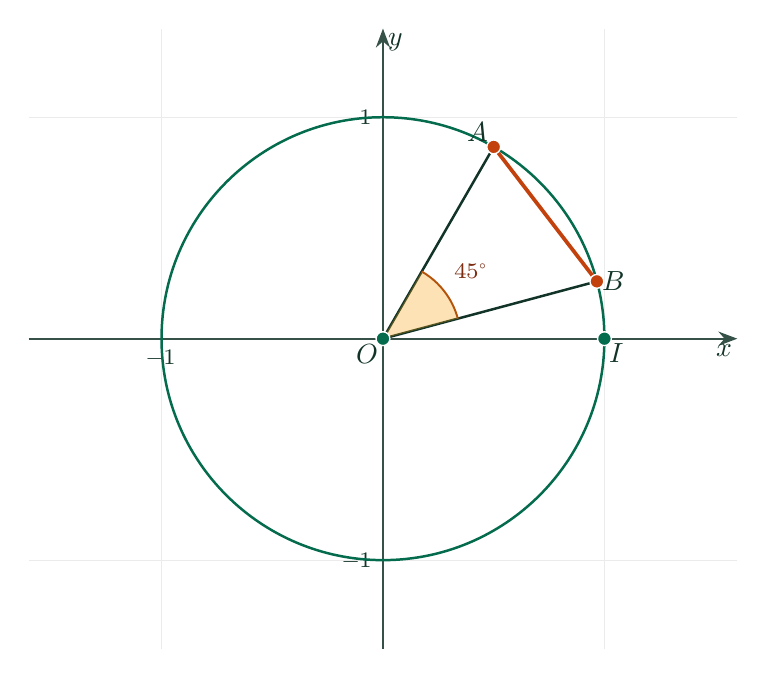
\begin{tikzpicture}[x=2.8125cm, y=2.8125cm]
\draw[gray!16, line width=0.4pt] (-1,-1.4) -- (-1,1.4) (0,-1.4) -- (0,1.4) (1,-1.4) -- (1,1.4);
\draw[gray!16, line width=0.4pt] (-1.6,-1) -- (1.6,-1) (-1.6,0) -- (1.6,0) (-1.6,1) -- (1.6,1);
\draw[ink!85, line width=0.7pt, -{Stealth[length=2.4mm]}] (-1.6,0) -- (1.6,0) node[anchor=north east, lab, font=\normalsize] {$x$};
\draw[ink!85, line width=0.7pt, -{Stealth[length=2.4mm]}] (0,-1.4) -- (0,1.4) node[anchor=north west, lab, font=\normalsize] {$y$};
\draw[ink!70] (-1,0.028444444444444446) -- (-1,-0.028444444444444446) node[below, lab, font=\footnotesize] {$-1$};
\draw[ink!70] (0.028444444444444446,-1) -- (-0.028444444444444446,-1) node[left, lab, font=\footnotesize] {$-1$};
\draw[ink!70] (0.028444444444444446,1) -- (-0.028444444444444446,1) node[left, lab, font=\footnotesize] {$1$};
\tkzDefPoint(0,0){O}
\tkzDefPoint(1,0){I}
\tkzDefPoint(1,0){tmp1}
\tkzDefPoint(0.5,0.866025){A}
\tkzDefPoint(0.965926,0.258819){B}
\begin{scope}
\clip (-1.6,-1.4) rectangle (1.6,1.4);
\tkzDrawCircle[draw={rgb,255:red,4;green,107;blue,77}, line width=0.9pt](O,tmp1)
\tkzDrawSegment[draw=ink, line width=0.90pt](O,A)
\tkzDrawSegment[draw=ink, line width=0.90pt](O,B)
\tkzDrawSegment[draw={rgb,255:red,194;green,65;blue,12}, line width=1.35pt](A,B)
\end{scope}
\tkzFillAngle[size=0.35, fill={rgb,255:red,245;green,158;blue,11}, fill opacity=0.3](B,O,A)
\tkzMarkAngle[size=0.35, draw={rgb,255:red,180;green,83;blue,9}, line width=0.7pt, mark=none](B,O,A)
\tkzLabelAngle[pos=0.499, text={rgb,255:red,124;green,45;blue,18}, font=\footnotesize](B,O,A){$45^{\circ}$}
\node[dot, fill={rgb,255:red,4;green,107;blue,77}] at (O) {};
\node[dot, fill={rgb,255:red,4;green,107;blue,77}] at (I) {};
\node[dot, fill={rgb,255:red,194;green,65;blue,12}] at (A) {};
\node[dot, fill={rgb,255:red,194;green,65;blue,12}] at (B) {};
\node[lab, font=\normalsize, anchor=north east] at (0,0) {$O$};
\node[lab, font=\normalsize, anchor=north west] at (1,0) {$I$};
\node[lab, font=\normalsize, anchor=south east] at (0.5,0.86603) {$A$};
\node[lab, font=\normalsize, anchor=west] at (0.96593,0.25882) {$B$};
\end{tikzpicture}
\end{document}
